\documentclass{article}
\usepackage{parskip}
\usepackage{pdfpages}
\usepackage[margin=.6in]{geometry}
\begin{document}
\section*{Schrodiner's Apology}
\label{sec:schrodiner_s_apology}
He was the first physisit to step into the "What is life?" question. He wrote an apology for not knowing any biology during his book on it.

\section*{Introduction}
\label{sec:introduction}
We accept evolution as the best explanation for the source of all life. Supposidly there was a last universal common ancestor (LUCA). Life is broken up into eukaryotes (multi cell life), archaea, and backteria (single cell life). This doesnt explain where that LUCA came from (the origin of all life).

\section*{When did life begin}
\label{sec:when_did_life_begin}
A stramatolite is a blob, rock looking thing in the ocean. Its layers of sediment mixed with layers of microbes. Autotrophs are bacteria near the top of the layer that take in sunlight and make organic compounds (like sugars). The next layer down has hertotrophs that use those sugars to create water and co2 that the autotrophs use. These two types alternate layers since they cycle the same stuff. Inside the layers in the stromatolites there are microcosms that represent life on earth.

When you cut open really old rocks they have similar layers to stromatolites which might make you think they might be dead stromatolites but those layers could be completely inorganic. Carbon 12/13 ratio is usually around 89:1 but life is better at metabolizing carbon 12. So if the carbon 12/13 ratio is different we can conclude that organisms were there to eat up the c12. So we can determine which of these layered rocks had life in them. They date back to about 3.5 billion years which gives us a sort of date for the origin of life. But at that point we already had complex life (able to photosynthesize) which means that life is much older that that. Earth is only 4.6 billion years old so life is really fucking old.

Microfossils would be an awesome find. But its really hard to find these super old rocks that haven't been disturbed (re-introduced into the rock cycle) which would destroy the microfossils in them. Its also very hard to tell what is a microfossil and what is just a crystal or other geologic figure. Our current oldest microfossil is around 3.4 billion years old. We thing its organic because it displays clustering behavior, it has messed up c12/c13 ratios within and without the cell, and sulfur isotope ratios are also messed up which implies it might have been metabolizing sulfur.

The oldest rocks with messed up c12/c13 ratios is on the island of akilia off the coast of Greenland at about 3.85 bya. We can also see other isotopes that get messed up by the presence of life that we can look at (see above sulfur comment).

The current evidence is that life evolved shortly after the late heavy bombardment (which happened at 4.1 bya). This could mean that life is very prevalent in the universe instead of just a lucky event.


\section*{Where did life begin?}
\label{sec:where_did_life_begin_}
DNA mutates; thats just what it does. There is a predictable and measurable rate of evolution based on those mutations in dna. By comparing genomes of organisms we can tell how close their common ancestor was, from doing this we build a tree of life.

We can track back dna to show that sharks branched out first and using the tree of life we can find that most early life was extremophiles.

\includepdf[pages=11]{slides}
We're pretty sure life evolved in water because water is hella important to life. Darwin thought that life may have evolved in a very warm tide pool randomly. We kind of dismiss this theory because concentrated UV rays might have messed that up.

\includepdf[pages=12]{slides}
For life to evolve we need some protection from UV rays which we can get deep in the ocean. Another point against the warm puddle theory is that the late heavy bombardment would have vaporized any life there unless it was living underground or deep in the sea.

\includepdf[pages=13]{slides}
\section*{How Did Life Begin?}
\label{sec:how_did_life_begin_}
Amino acids are the building blocks of life. They have a carbon backbone which is why we call ourselves carbon based life forms. We really are only made of about 20 amino acids. We can syntesize 12 of them so we only really need the other 8 from our diet. We combine these amino acids into more complicated molecules, usually proteins. Long chains of molecules can be formed randomly.

\includepdf[pages=14]{slides}
Proteins are formed from long chain of amino acids taht get folded up into 3D shapes. Proteins are primarily used for catalyzing complex metabolic reactions. Most molecules rest in a comfortable state so we have to push on them to form a gap where other molecules can snap into it. This can happen on its own but is very slow (too slow for life). Enzymes (a type of protine) speeds up this process. They provide pockets for the two molecules that we want to combine. To get into those pockets they have to bend and snap into place. They do this because the nearby water molecules that keep coliding with them. A water molecule bumps into a molecule and makes it bend into the protine. At this point ATP comes into play that can harnes this mechanical energy.

\includepdf[pages=15]{slides}
Proteins are also used in the replication of dna. One splits the dna in half (into 2 single helixes). Things are duplicated and then its zipped together to form a new strand of dna.

\includepdf[pages=16]{slides}
Amino acids are all over the place. Even in space, on asteroids. They need a ton of time to combine into these weird things called life.

\includepdf[pages=17]{slides}
When we were first looking at ancient earth we looked at all the sedimentary layers. Physists eventually got involved and found that the earth can't be older than the sun. So they tried to calculate the age of the sun. They did this by looking at the size of the sun and assuming that it created energy through gravity. He didn't know that it worked through fusion so his age was way off. They we looked at how long it would have taken molten earth to cool to the state that its at. This ignored radioactive rocks in earth which give off heat that extended the age of earth.

Biologists were arguing that the age of the earth was much older than that. Darwin's original Theory of Evolution stated that the earth must be billions of years old but the physists made him remove that.

\includepdf[pages=18]{slides}
Eventually we learned more about earth and the geologists got to a number that more closely matched what the biologists knew.

\includepdf[pages=19]{slides}
As radioactive elements in a rock decay they do so at a steady rate. This allows us to look at ratios between two elements and that will tell us how long it has been since that rock solidified (else the gases would have escaped).

It is believed that a mars sized body collided with earth near is birth which caused it to break apart which formed the moon. If we look at the oldest rocks on the moon we see that they are roughly the same age.

We can also see that stars that are similar to the sun brighten at a constant rate over time. This lets us look at other stars in the system (that are similar to the sun) and age them. From this we get that the sun is about as old a earth.

\includepdf[pages=20]{slides}
When the universe first formed it really only made hydrogen and helium. It is in the cores of the stars that heavier elements are formed (still only about 2\% heavier elements).

Eventually rocks are formed by electrostatic and gravitational pull making larger and larger clumps of molecules.

\includepdf[pages=21]{slides}
Rocky/metalic planets form near the center of solar system since they are made of heavier elements (and icey elements would have evaporated in the heat). At first it had no atmosphere (it isn't big enough to have the pull to do it like jupier does). We get our atmosphere from water vapor being spewed by volcanoes (we think). Another theory about the origin of the atmosphere is that the thing that collided with us did so with such force that it released a bunch of water that was sealed inside rocks.

\includepdf[pages=22]{slides}
\includepdf[pages=23]{slides}
These two guys put what they thought was the atmosphere of early earth and waited. Eventaully amino acids formed. The problem with this is that the early atmosphere was actaully co2 based. Out current experiments show that the kind of amino acids formed depends on the ratio of carbon in the air.

Moral of the story amino acids are easy to produce.

\includepdf[pages=24]{slides}
There are a bunch of different natural path ways that we need to explore that could have resulted in the change between animo acids to true biology.

\includepdf[pages=25]{slides}
Modern dna doesnt replicate itself without proteins. On the other side we know that proteins cannot be made without dna. The solution to this is that RNA can behave like a protein to help rna self replicate without the use of proteins. This lead to the notion that early life was just rna called the rna world.

\includepdf[pages=26]{slides}
You have some rna bases floating around in water (you can made these randomly). Within zircon chips that are hella old (near the beginning of earth) there are these inclusions of "clay". If you add this clays to the water with rna bases the clay spontaneously acts like an enzyme so the rna bases slots into these pockets in the clay by random chance and snap together.

\includepdf[pages=27-31]{slides}
We now have short strands of base pairs just floating around. These can clip together or serve as the substrate to facilitate other strands to snap together.

The ocean has tons of these clay grains and rna chunks floating around we can see that there are tons of combinations being formed which eventually forms a strand of rna long enough to self replicate (165 bases). At this point grown becomes exponential growth.

\includepdf[pages=32]{slides}
We run into another chicken and egg problem with the cell membrane did if form before or after is genes. If you put a bunch of lipids in water they will form a cell membrane spontaneously because they have hydrophobic tails that slot themselves on the inside. If you run this experiment in the presense of the zircon clay it will act as a catalyst to speed up the formation of cells.

\includepdf[pages=33]{slides}
These cell membranes can form randomly they can form around some rna strands. This makese the chemistry in the cell concentrated until the cell swells and splits into daughter cell. This concentration speeds up the process. Because this replicates at an exponential speed it dominates over everything else.

\includepdf[pages=34]{slides}
DNA is much more solid than RNA which is more prone to errors.

\includepdf[pages=35]{slides}
Summary:
\begin{itemize}
	\item amino acids are really easy to make
	\item clay that is super common can act as a catalyst to form rna
	\item rna links together to become large enough to self replicate
	\item cell membranes can form randomly around rna strands
	\item dna evolves from rna and is better at continuing so it takes over
\end{itemize}




\end{document}

